\documentclass[twoside]{article}

%%%% This is a link to the packages that should work %%%
% https://math.nist.gov/~BMiller/LaTeXML/manual/included.bindings/ %

%%% Working %%%
	\usepackage{latexml}
	\usepackage{amsmath,amssymb,amsthm}
	\usepackage{tikz}
	        \usetikzlibrary{automata,positioning}
	        \tikzset{>=stealth}
	\usepackage{graphicx}
	\usepackage{calc,ifthen}
	\usepackage{lscape}
	\usepackage[table]{xcolor}
	\usepackage{multicol,tabularx}
	\usepackage{colortbl}
	\usepackage{mathrsfs,xfrac}
    \usepackage{bbding}
    \usepackage{newtxmath}
    \usepackage{newtxtext}
    \usepackage{pgfplots}
    \pgfplotsset{compat=newest}
    \usepackage{caption}
    \usepackage{subcaption}
    \usepackage{titling}


%%%% Document Colors
    % \colorlet{Mycolor1}{green!10!orange}
    % \definecolor{Mycolor2}{HTML}{00F9DE}
    \colorlet{accent}{blue!70!black}
    \colorlet{secondaryaccent}{red!50!black}
    \colorlet{tertiaryaccent}{green!50!black}
    \colorlet{background}{accent!5}
    \colorlet{S_background}{secondaryaccent!5}
    \colorlet{T_background}{tertiaryaccent!5}
    \definecolor{safety}{HTML}{D6C01A}
    \definecolor{PotsdamMaroon}{HTML}{8A1538}
    \definecolor{PotsdamGray}{HTML}{A2AAAD}
    \definecolor{WCSUBlue}{HTML}{002856}
    \definecolor{WCSUOrange}{HTML}{FF4D00}

%%%% Layout Commands %%%%
    \pagestyle{myheadings}
    \usepackage{geometry}
    \geometry{
        inner=0.75in,
        outer=0.75in,
        top=1in,
        bottom=0.75in
    }
    % this tells LaTeX to look in this directory 
    % if it doesn't find the images else where
    \graphicspath{ {../images/} }

% New Commands and Theorem Environments
    % Rewritten emphasis command
    \DeclareTextFontCommand{\emph}{\em\bfseries\color{secondaryaccent}}

    % Misc. New Symbols/Commands
    \newcommand{\accentcheckmark}{\textcolor{accent}{\CheckmarkBold}}
    \newcommand{\accentXbrush}{\textcolor{secondaryaccent}{\XSolidBrush}}
    \newcommand{\redheart}{\textcolor{secondaryaccent}{\varheartsuit}}
    \newcommand{\reddiamond}{\textcolor{secondaryaccent}{\vardiamondsuit}}


%%% Testing %%%
    \usepackage{fancyvrb}
\usepackage{listings}

\lstset{
  basicstyle=\ttfamily,
  linewidth=5in,
  breaklines,
  numbers=left
}




%%% Throws a minor error %%%
% \usepackage{hanging}
% \usepackage{lipsum} This is supposed to work but is causing compilation to hang, the AI answer is that newer Latex3 implementations may not work.
% \usepackage{fdsymbol}
% \usepackage{tcolorbox} This is another onbe that is supposed to be supported but is causing issues
% \usepackage{minted} not supported and generally problematic





\newcounter{test}
\setcounter{test}{5}


%%%% Hyper reference package information %%%%
    \usepackage[
            pdftitle={Hello World},
            pdfauthor={Chuck Rocca},
            pdfproducer={Latex with hyperref},
            pdflang={en-US},
            linkcolor=blue!70!black,
            colorlinks=true,
            urlcolor=blue!70!black
        ]{hyperref}


\title{Hello World}
\author{Chuck Rocca}

\begin{document}


\maketitle

\markboth{\thetitle}{\theauthor}


\begin{abstract}
	Here we will put together an even simpler document.  We begin by adding no packages and then carefully introduce them compiling a little at a time.
\end{abstract}

\section{First Section}

Hello World!!!

\section{Second Section}

\subsection{A Subsection}

Here is a subsection!!!

\subsection{Another Subsection}

Here is another subsection!!!

\section{Let's Try some Math}

Here is an inline equation: \(x^2+3x+7=10\).  Here is the same equation displayed: \[x^2+3x+7=10.\] Then we can use a stacked equation to show solving this:
\begin{align}
	x^2+3x+7=10 &\Rightarrow x^2+3x=3\\
		&\Rightarrow x^2+3x+\frac{9}{4}=5\frac{1}{4}\\
		&\Rightarrow \left(x+\frac{3}{2}\right)^2=\pm\sqrt{5\frac{1}{4}}\\
		&\Rightarrow x=-\frac{3}{2}\pm\sqrt{5\frac{1}{4}}\ .
\end{align}
What if we use special symbols like \(\mathbb{N}\) or \(\mathfrak{N}\)?  Yes, both of those worked well.  What about \(\mathcal{P}\) and \(\sfrac{2}{3}\) and \XSolidBrush?  Yep, that worked too.

\section{Let's Add a Diagram}
Let us add in \verb|\usepackage{tikz}| and make a diagram.  Before even making a diagram we note that the compile time increases significantly while \verb|latexml| parses what to do with \verb|tikz|.  Now here is a small figure:
\begin{figure}[hbpt]
	\centering
	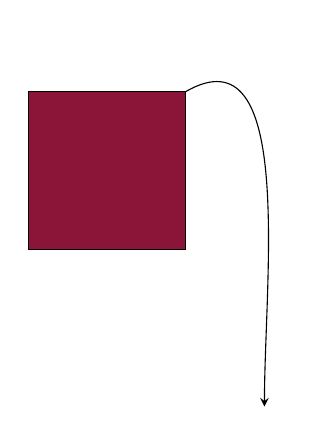
\begin{tikzpicture}
		\draw[fill=PotsdamMaroon] (0,0) rectangle (2,2);
		\draw[->] (2,2) to[out=30,in=90] (3,-2);
	\end{tikzpicture}
	\caption{Our First Diagram}
	\label{fig:our_first_diagram}
\end{figure}


\begin{figure}[htbp]
    \centering
    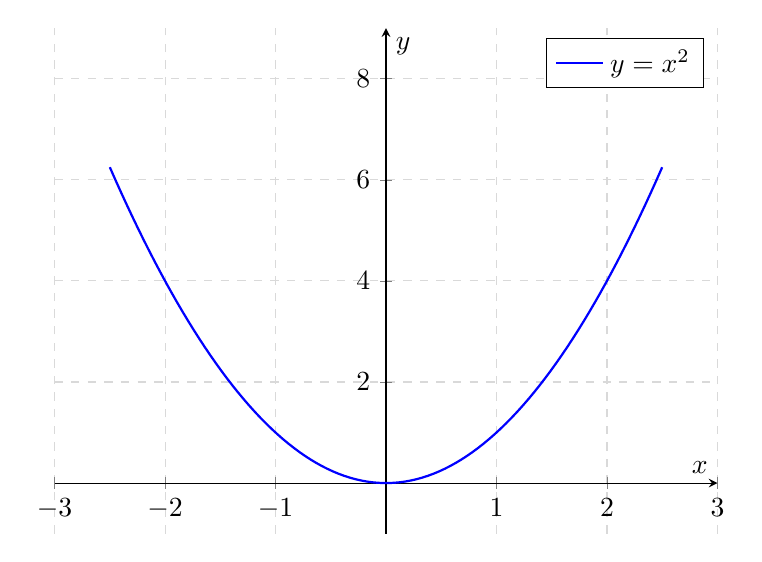
\begin{tikzpicture}
        \begin{axis}[
            axis lines = middle,    % Places axes in the center forming a cross
            xlabel = {$x$},         % Label for the x-axis
            ylabel = {$y$},         % Label for the y-axis
            xmin = -3, xmax = 3,    % Minimum and maximum x-axis limits
            ymin = -1, ymax = 9,    % Minimum and maximum y-axis limits
            grid = both,            % Displays both major and minor grid lines
            grid style = {dashed, gray!30},
            width = 10cm,           % Width of the plot area
            height = 8cm            % Height of the plot area
        ]
            % Plotting the parabola
            \addplot [
                domain = -2.5:2.5,  % Range over which x is evaluated
                samples = 100,      % Number of calculated points (high = smooth)
                color = blue,       % Line color
                thick               % Line thickness
            ] {x^2};                % The mathematical function
            
            % Optional: Add a legend entry for the curve
            \addlegendentry{$y = x^2$}
            
        \end{axis}
    \end{tikzpicture}
    \caption{Parabola plot using PGFPlots. (from Gemini)}
    \label{fig:parabola}
\end{figure}

\section{Now an Image}
	\begin{figure}[hbpt]
		\centering
			
\includegraphics[alt={zombie}]{zombie.png}
		\caption{A Zombie}
		\label{fig:zombie}
	\end{figure}

	\begin{figure}[hbpt]
		\begin{subfigure}{0.45\textwidth}
			\centering
				
\includegraphics[alt={zombie}]{zombie.png}
			\caption{Zombie One}
			\label{fig:zombie_one}
		\end{subfigure}
		\begin{subfigure}{0.45\textwidth}
			\centering
				
\includegraphics[alt={zombie}]{zombie.png}
			\caption{Zombie Two}
			\label{fig:zombie_two}
		\end{subfigure}
		\caption{Two Zombies}
		\label{fig:two_zombies}
	\end{figure}

\section{Miscellaneous Tests}
\iflatexml
	This is a test
\else
	This is another test
\fi

\ifthenelse{\thetest=5}{then clause}{else clause}

\begin{table}[hbpt]
	\centering
	\caption{The First 25 Prime Numbers in Alternating Colors}
	\label{tab:colored_primes}
	% \rowcolors{start_row}{odd_color}{even_color}
	\rowcolors{1}{gray!20}{blue!15} 
	\begin{tabular}{|*{5}{c|}}
	\hline
	2  & 3  & 5  & 7  & 11 \\ \hline
	13 & 17 & 19 & 23 & 29 \\ \hline
	31 & 37 & 41 & 43 & 47 \\ \hline
	53 & 59 & 61 & 67 & 71 \\ \hline
	73 & 79 & 83 & 89 & 97 \\ \hline
	\end{tabular}
\end{table}

\begin{landscape}
This is in landscape in the PDF, the HTML understandably ignores this.
\end{landscape}

\begin{multicols}{2}
	This is a test. This should split the text into multiple columns.  It may be hard to see this in action without sufficient text.  This is why the lipsum package is helpful.  It looks like the HTML produced by LatexML also ignores the multicols environment, this also makes since.
\end{multicols}

\begin{table}[hpbt]
	\centering
	\rowcolors[\hline]{3}{green}{yellow} \arrayrulecolor{red}
	\begin{tabular}{ll}
	test & row \thetest\\
	test & row \thetest\\
	test & row \thetest\\
	test & row \thetest\\
	\arrayrulecolor{black}
	test & row \thetest\\
	test & row \thetest\\
	\rowcolor{blue}
	test & row \thetest\\
	test & row \thetest\\
	\hiderowcolors
	test & row \thetest\\
	test & row \thetest\\
	\showrowcolors
	test & row \thetest\\
	test & row \thetest\\
	\multicolumn{1}%
	{>{\columncolor{red}}l}{test} & row \thetest\\
	\end{tabular}
	\caption{Example from colortbl manual}
	\label{table:example_from_colortbl_manual}
\end{table}
I should check that cross references work right like for figures \ref{fig:our_first_diagram} and \ref{fig:zombie} and tables \ref{tab:colored_primes} and \ref{table:example_from_colortbl_manual}.


\begin{lstlisting}[language=bash]
lualatex Hello_World
latexml Hello_World.tex --dest=Hello_Latexml.xml
latexmlpost Hello_latexml.xml --dest=Hello_latexml.html --javascript="https://cdn.jsdelivr.net/npm/mathjax@3/es5/tex-mml-chtml.js?config=MML_HTMLorMML" --split --splitat=section --navigationtoc=context --css=andy-navbar.css --css=normalize.css --urlstyle=file --timestamp=0 --javascript=andy-navbar.js
\end{lstlisting}

\section{Home Built or Defined Macros}

\(\redheart\)
\(\reddiamond\)
\accentcheckmark, 
\accentXbrush

\section{Notes:}
LatexML does not seem to like the document meta data.  This supports the idea that there should be two shells, one with metadata and one without.  The only problem with this is that the alt text in tikz seems to only be recognized when the metadata is present and compiling with lualatex.  This supports the view that it may be best practices to create diagrams separately and then import them.  Within the document the \verb|\iflatexml| command seems to work fine as long as the compiler can find \verb|latexml.sty|.  So far following the instructions at this site \url{https://hackmd.io/@UoL-IWG/latexml} has LatexML working like a champ; the question is about what packages this can handle.  There is also important information in the GitHub repository for the \LaTeX ML project: \url{https://github.com/brucemiller/LaTeXML}.  The package minted continues to be an issue, it is not supported natively by \LaTeX ML or tex4ht and is not listed as compatible with the work from the \LaTeX\/ Tagging project; we need to learn fancyvrb.  Tried fancyvrb and listings and listings seems to be the better of the two.  In listings look at the language options.

Notes from June 24th.  I adjusted the css files from \url{https://hackmd.io/@UoL-IWG/latexml} to elliminate some messy overlap with the navigation elements.



\end{document}